\documentclass[crop=false, class=memoir]{standalone}
\usepackage[utf8]{inputenc}%Nødvendig for danske bogstaver
\usepackage[danish]{babel}%Sørger for at ting LaTeX gør automatisk er på dansk
\usepackage{csquotes}
\usepackage{geometry}%Til opsætning af siden
\geometry{lmargin = 2.5cm,rmargin = 2.5cm}%sætter begge magner
\usepackage{lipsum}%Fyldtekst, til brug under test af layoutet
\usepackage{float}
\usepackage{graphicx}%Tillader grafik
\usepackage{epstopdf}%Tillader eps filer
\usepackage{marginnote}% Noter i margen
\interfootnotelinepenalty=10000 %undgår at fodnoter bliver spilittet op.
\usepackage[sorting=none]{biblatex}
\addbibresource{litteratur.bib}
\usepackage[hidelinks]{hyperref}%Tillader links
\usepackage{subcaption} % Tillader underfigurer
\usepackage[font={small,sl}]{caption}	% Caption med skrå tekst ikke kursiv

\usepackage{xcolor} %Bruges til farver
\usepackage{forloop} %Bruges til nemmere for loops

\newcounter{opgave}[chapter] %Definerer opgavenumrene og hvornår de nulstilles
\renewcommand{\theopgave}{\thechapter.\arabic{opgave}} %Definerer udseende af opgavenummereringen
\newcounter{delopgave}[opgave] %Definerer delopgavenumrene
\newcounter{lvl} %Definerer en "variabel" til senere brug

\definecolor{markerColor}{rgb}{0.0745098039, 0.262745098, 0.584313725} %Definerer farven af markøren
\newcommand{\markerSymbol}{\ensuremath{\bullet}} %Definerer tegnet for markøren
\newlength{\markerLength} %Definerer en ny længde
\settowidth{\markerLength}{\markerSymbol} %Sætter den nye længde til bredden af markøren

\newenvironment{opgave}[2][0]{%Definerer det nye enviroment, hvor sværhedsgraden er den første parameter med en default på 0
\newcommand{\opg}{\refstepcounter{delopgave}\par\vspace{0.1cm}\noindent\textbf{\thedelopgave)\space}}%Definerer kommando til delopgave
\refstepcounter{opgave}%Forøger opgavenummer med 1 og gør den mulig at referere til
\setcounter{lvl}{#1}%Sætter "variablen" lvl lig med angivelsen af sværhedsgraden
\noindent\hspace*{-0.75em}\hspace*{-\value{lvl}\markerLength}\forloop{lvl}{0}{\value{lvl}<#1}{{\color{markerColor}\markerSymbol}}\hspace*{0.75em}%Sætter et antal af markører svarende til sværhedsgraden
\textbf{Opgave \theopgave : #2}\newline\nopagebreak\ignorespaces}{\bigskip} %Angiver udseende af titlen på opgaverne samt mellemrummet mellem opgaver



\usepackage{mathtools}%Værktøjer til at skrive ligninger
\renewcommand{\phi}{\varphi}%Vi bruger varphi
\renewcommand{\epsilon}{\varepsilon}%Vi bruger varepsilon
\usepackage{physics}%En samling matematikmakroer til brug i fysiske ligninger
\usepackage{braket}%Simplere kommandoer til bra-ket-notation
\usepackage{siunitx}%Pakke der håndterer SI enheder godt
\DeclareSIUnit\clight{\text{\ensuremath{c}}} % Lysets fart i vakuum som c og ikke c_0
\usepackage{chemmacros}
\usechemmodule{isotopes}
\usepackage{tikz}
\usepackage[danish]{cleveref}
\usepackage{nicefrac}
% \renewcommand{\ref}[1]{\cref{#1}}
\creflabelformat{equation}{#2(#1)#3}
\crefrangelabelformat{equation}{#3(#1)#4 to #5(#2)#6}
\crefname{equation}{ligning}{ligningerne}
\Crefname{equation}{Ligning}{Ligningerne}
\crefname{section}{afsnit}{afsnitene}
\Crefname{section}{Afsnit}{Afsnitene}
\crefname{figure}{figur}{figurene}
\Crefname{figure}{Figur}{Figurene}
\crefname{table}{tabel}{tabellerne}
\Crefname{table}{Tabel}{Tabellerne}
\crefname{opgave}{opgave}{opgaverne}
\Crefname{opgave}{Opgave}{Opgaverne}
\crefname{delopgave}{delopgave}{delopgaverne}
\Crefname{delopgave}{Delopgave}{Delopgaverne}

\newcommand{\eqbox}[1]{\begin{empheq}[box=\fbox]{align}
	\begin{split}
	#1
	\end{split}
\end{empheq}}

\newcommand{\kb}{\ensuremath{k_\textsc{b}}}

\DeclareSIUnit{\parsec}{pc}
\DeclareSIUnit{\lightyear}{ly}
\DeclareSIUnit{\astronomicalunit}{AU}
\DeclareSIUnit{\year}{yr}
\DeclareSIUnit{\solarmass}{M_\odot}
\DeclareSIUnit{\solarradius}{R_\odot}
\DeclareSIUnit{\solarluminosity}{L_\odot}
\DeclareSIUnit{\solartemperature}{T_\odot}
\DeclareSIUnit{\earthmass}{M_\oplus}
\DeclareSIUnit{\earthradius}{R_\oplus}
\DeclareSIUnit{\jupitermass}{M_J}

% Infobokse og lignende
% http://mirrors.dotsrc.org/ctan/graphics/awesomebox/awesomebox.pdf
% \usepackage{awesomebox}


% Egen infobokse (virker kun med begrænsede symboler)

\usepackage[framemethod=tikz]{mdframed}
\usetikzlibrary{calc}
\usepackage{kantlipsum}

\usepackage[tikz]{bclogo}

\tikzset{
    % lampsymbol/.style={scale=2,overlay}
    % lampsymbol/.pic={\centering\tikz[scale=5]\node[scale=10,rotate=30]{\bclampe}}.style={scale=2,overlay}
    infosymbol/.style={scale=2,overlay}
}

\newmdenv[
    hidealllines=true,
    nobreak,
    middlelinewidth=.8pt,
    backgroundcolor=blue!10,
    frametitlefont=\bfseries,
    leftmargin=.3cm, rightmargin=.3cm, innerleftmargin=2cm,
    roundcorner=5pt,
    % skipabove=\topsep,skipbelow=\topsep,
    singleextra={\path let \p1=(P), \p2=(O) in ($(\x2,0)+0.92*(1.1,\y1)$) node[infosymbol] {\bcinfo};},
    % singleextra={\path let \p1=(P), \p2=(O) in ($(\x2,0)+0.5*(2,\y1)$) node[infosymbol] {\bcinfo};},
]{info}

% Skal bruges som
% \begin{info}[frametitle={Titel}]
%     Tekst
% \end{info}
\usepackage{import}
\begin{document}
\chapter{Elektromagnetisme} \label{chap:elektro_opg}
\subsection*{Elektrostatik}
\begin{opgave}[1]{Coulombkraften}
    To ladninger, $q$ og $Q$ har en indbyrdes afstand $r$ til hinanden.
    \opg Bestem Coulombkraften fra den ene ladning på den anden i hvert af følgende tilfælde:
    \begin{enumerate}
        \item $r = \SI{1,00}{\metre}$, $q = \SI{1,00}{\coulomb}$ og $Q = \SI{1,00}{\coulomb}$
        \item $r = \SI{1,00}{\metre}$, $q = \SI{1,00}{\coulomb}$ og $Q = \SI{-1,00}{\coulomb}$
        \item $r = \SI{1,00}{\metre}$, $q = \SI{1,00}{\coulomb}$ og $Q = \SI{2,00}{\coulomb}$
        \item $r = \SI{2,00}{\metre}$, $q = \SI{1,00}{\coulomb}$ og $Q = \SI{1,00}{\coulomb}$
    \end{enumerate}
    \opg Beskriv med ord hvad der sker med Coulombkraften når den ene ladning skifter fortegn, dens størrelse fordobles og når ladningernes indbyrdes afstand fordobles.
    \opg Brug Newtons anden lov, $\va{F}=m\va{a}$, til at bestemme accelerationen af hver ladning i tilfælde 1. Ladningernes masse er $m_1 = \SI{1,00}{\kilo\gram}$ og $m_2 = \SI{2,00}{\kilo\gram}$.
    \opg Bestem accelerationen af ladning 1 i tilfælde 2-4.
    \opg Beskriv med ord hvad der sker når ladningerne frigives i de fire tilfælde og sammenlign dem.
\end{opgave}

\begin{opgave}[2]{Tre ladninger på en linje}
    To punktladninger med ladning $+q$ befinder sig ved positioner $x=-a$ og $x=a$.
    \opg Bestem kraften på en anden ladning $+Q$ som funktion af dens position langs $x$-aksen.
    \opg Tegn en graf over kraften som funktion af position, og kommenter den generelle opførsel.
    \opg Hvordan vil ladningen bevæge sig når den er ved $x=0$?
    \opg For $x\gg a$, approksimer udtrykket for kraften. \textit{Hint: Hvad sker der hvis man lægger et lille tal til et stort tal?}
\end{opgave}

\begin{opgave}[1]{Firkantet ladningskonfiguration}
Betragt fire punktladninger sat i et kvadratisk mønster. Vi vil nu undersøge hvilken retning en testladning $Q$ skubbes. Tegn retningen som $Q$ vil bevæge sig i de tre tilfælde vist i \cref{em:fig:ladning_i_firkant}.
\begin{figure}[]
    \centering
    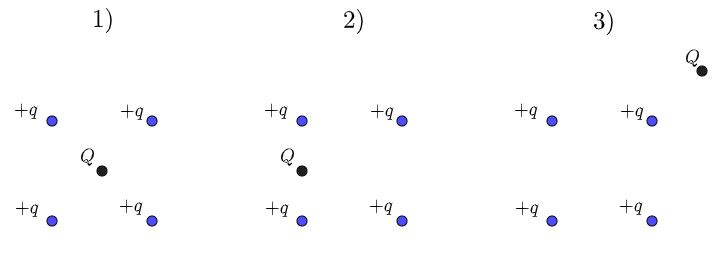
\includegraphics[width=.9\textwidth]{Elektro/Elekfig/firkant.JPG}
    \caption{Tre forskellige positioner for Q.}
    \label{em:fig:ladning_i_firkant}
\end{figure}
\end{opgave}

\begin{opgave}[2]{Fluxopgave I} \label{em:opg:flux1}%
Betragt en uendelig lang linjeladning $\lambda$. Linjeladningen udspænder E-feltet $\va{E}=\lambda/(2\pi r \epsilon_0)\vu{s}$, hvor $\vu{s}$ er en enhedsvektor, der peger vinkelret væk fra linjen (og variablen $r$, er også den vinkelrette distance væk fra linjen). For illustration af Gaussoverfladen se \cref{em:fig:flux1}.
\opg Bestem fluxen igennem en cylinder Gaussoverflade med radius $R$ og længde $L$. \emph{Hint: Er E-feltet konstant langs noget af overfladen?}
\opg Bestem dernæst fluxen igennem en cylinder Gaussoverflade med radius $2R$ og længde $L$
\opg Bestem tilsidst fluxen igennem en cylinder Gaussoverflade med radius $R$ og længde $2L$
\opg Forklar hvorfor fluxen er større i det ene tilfælde og uændret i det andet tilfælde.
    \begin{figure}[]
        \centering
        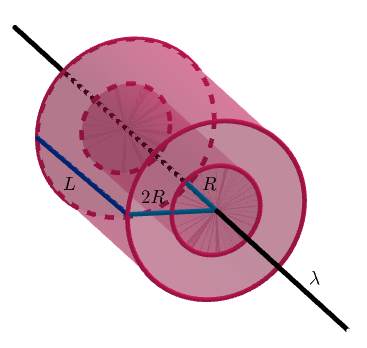
\includegraphics[width=.52\textwidth]{Elektro/Elekfig/cylinder.PNG}
        \caption{Cylinderen til spørgsmål 1 og 2 i \cref{em:opg:flux1}.}
        \label{em:fig:flux1}
    \end{figure}
\end{opgave}

\begin{opgave}[2]{Fluxopgave II}
Betragt to parallele plader, der hver har en konstant overfladeladningstæthed $\sigma$. En enkelt plade udspænder E-feltet $\va{E}=(\sigma/2)\vu{n}$.
\opg Bestem E-feltet under, imellem og over de to plader.

\opg Vi vil nu prøve at regne fluxen på dette E-felt. Brug kassen markeret 1) i \cref{em:fig:flux2} som  Gaussoverflade og bestem fluxen.
\opg Brug kassen markeret 2) i \cref{em:fig:flux2} som  Gaussoverflade og bestem fluxen.
\opg Forklar hvorfor fluxen er dobbelt så stor i 2) end i 1).
    \begin{figure}[]
        \centering
        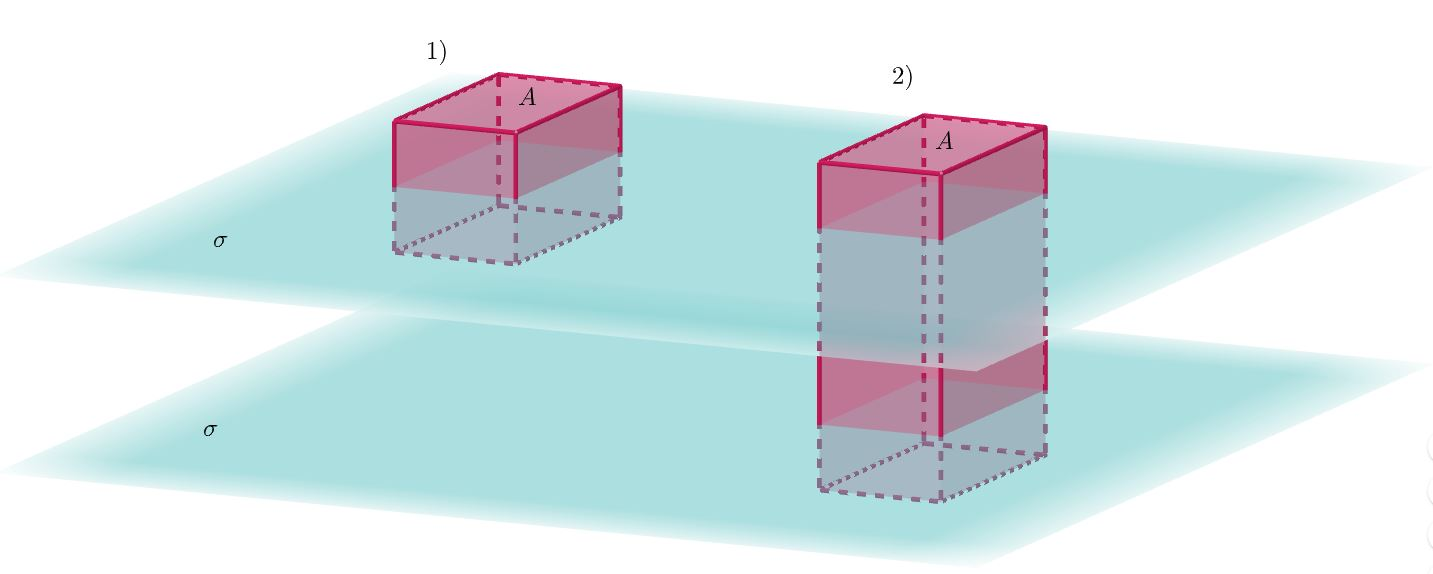
\includegraphics[width=\textwidth]{Elektro/Elekfig/tokapacitor.JPG}
        \caption{To forskellige Gaussoverflader.}
        \label{em:fig:flux2}
    \end{figure}
\end{opgave}

\begin{opgave}[3]{Uendelig lang ladet linje}
    For at beregne det elektriske felt overalt i rummet fra en uendelig lang ladet linje med konstant linjeladning $\lambda$ bruges Gauss' lov.
    \opg Argumenter for at det elektriske felt peger direkte væk fra linjen overalt i rummet. (Anvend hvad vi har lært omkring en linjeladning i 2D)
    \opg Argumenter for at E-feltet er rotationssymmetrisk omkring linjeladningen.
    \opg Hvis $\vu{s}$ er en vektor, som peger vinkelret væk fra linjeladningen, så er E-feltet $\va{E}=|E|\vu{s}$. Anvend dette og rotationssymmetrien til at argumentere for, at en cylinder Gaussoverflade omkring linjeladningen er en god ide. 
    \opg Giv din cylinder radius r og længde L. Det lukkede integral i Gauss' lov $\oint\va{E}\cdot\dd{\va{a}}$ kan skrives som en sum af hver de 3 overflade en cylinder har. Lad $S_1$ angive den krumme overflade, og henholdsvis $S_2$ og $S_3$ angive de to endestykker. Løs integralet
    \begin{align*}
        \oint_S \va E \cdot \dd{\va a} = \int_{S_1} \va E \cdot \dd{\va a} + \int_{S_2} \va E \cdot \dd{\va a} + \int_{S_3} \va E \cdot \dd{\va a}.
    \end{align*}
    \opg Brug nu Gauss' lov til at bestemme det elektriske felt overalt i rummet. \\
    \emph{Hint}: Længden af cylinderen skulle gerne gå ud, så det endelige udtryk kun afhænger af $\lambda$, $r$ og nogle konstanter.
\end{opgave}

\begin{opgave}[3]{Ladet kugle}
    En solid ladet kugle med radius $R$ har en konstant volumeladning $\rho$ for $r<R$ og $\rho=0$ for $r>R$, hvor $r$ er afstanden fra kuglens centrum.
    \opg Anvend hvad vi ved om en sfære overfladningsladning til at redegøre for hvilken vej E-feltet peger udenfor og indenfor kuglen.
    \opg Brug Gauss' lov til at bestemme det elektriske felt $\va{E}$ for $r>R$.
    \opg Brug Gauss' lov til at bestemme det elektriske felt $\va{E}$ for $r<R$. \emph{Hint}: Det er vigtigt, at huske at $Q_{enc}$ ikke er konstant inde i kuglen.
\end{opgave}

\begin{opgave}[3]{Cylinder ladningskonfigurationer}
    En uendelig lang hul cylinder med radius $R$ har en konstant overfladeladning $\sigma$.
    \opg Split overfladen af cylinderen op i uendelig lange linjeladninger og argumenter for retningen af E-feltet udenfor og inden i cylinderen. \emph{Hint: Det kan hjælpe at kigge 2-dimensionalt på cylinderen (altså en cirkel) og se hvert punkt på cirklen som en uendelig lang linjeladning}.
    \opg Anvend, at cylinderen er rotationssymmetrisk og bestem E-feltet for $r>R$.
    \opg Bestem dernæst E-feltet for $r<R$.
    \newline
    Dernæst vil vi kigge på en uendelig lang solid cylinder med radius R, der har en konstant volumeladning $\rho$.
    \opg Split den solide cylinder op i cylinder-overflader og argumenter for E-feltets retning udenfor og inden i den solide cylinder.
    \opg Anvend rotationssymmetri og bestem E-feltet for $r>R$.
    \opg Bestem til sidst E-feltet for $r>R$. \emph{Hint}: $Q_\textup{inde}$ er ikke konstant inde i den solide cylinder.
\end{opgave}

\begin{opgave}[4]{Endelig linjeladning}
I denne opgave vil vi prøve at kaste os over de ladningstæthedsintegraler, der kræver at man kender til integration. Betragt en konstant linjeladning $\lambda$ langs x-aksen med en længde på L, sådan at linjeladningens venstre ende er i origo. Vi vil nu finde E-feltet i en position $(y,0)$. Se figur \ref{endeliglinje}.
\opg Opskriv $\va{R}$.
\opg Opskriv nu $\vu{R}$. \emph{Hint}: En enhedsvektor kan altid skrives som $\vu{n}=\va{n}/|n|$.
\opg Opskriv integralet for E-feltet.
\opg Integralet kan deles op i to (i $\vu{x}$ og $\vu{y}$ retningen). Løsningen af det ene integrale er lidt nemmere, hvis man kan ens integrations tricks. Anvend integration af substitution til at bestemme integralet langs x-aksen.
\opg Det andet integrale er mere indviklet. Anvend substitutionen $x=y\tan({u})$, og at $1+\tan({u})^2=1/cos({u})^2$ og $\sin({\tan^{-1}(L/y)})=L/(\sqrt{L^2+y^2})$ til at bestemme integralet langs z-aksen. Hvis man har løst begge integraler, så har man fundet et udtryk for E-feltet: tillykke.
    \begin{figure}
        \centering
        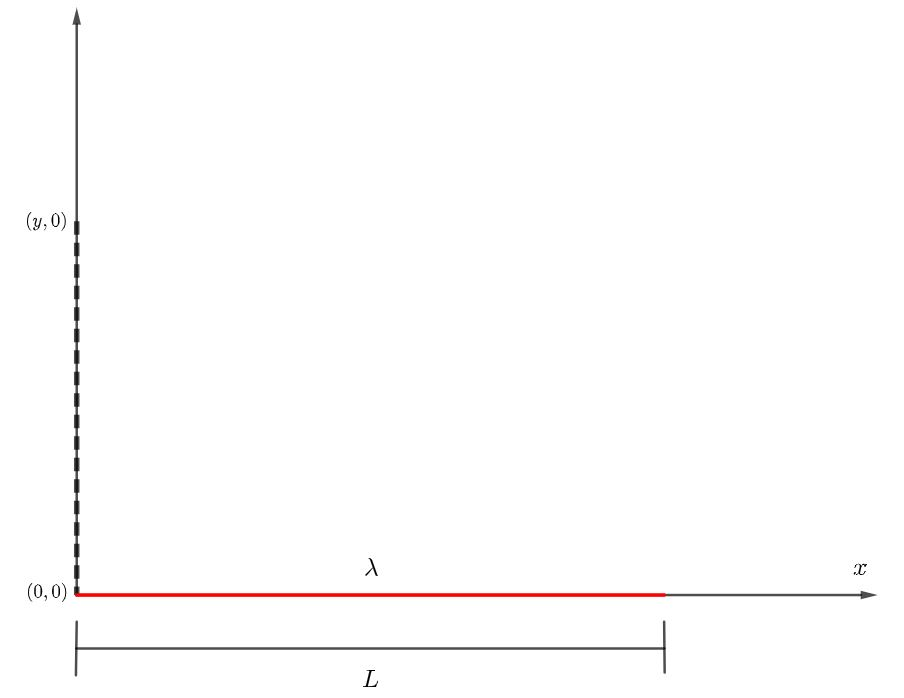
\includegraphics[scale=0.5]{Elektro/Elekfig/endeliglinje.JPG}
        \caption{}
        \label{endeliglinje}
    \end{figure}
\end{opgave}


\subsection*{Magnetisme}
\begin{opgave}[3]{Solenoiden}
    En måde at fremstille et (approksimativt) uniformt magnetfelt er ved brug af en solenoide, som illustreret i figur \ref{fig:solenoide}, hvori en strøm med strømstyrken $I$ løber. Det antages at solenoiden befinder sig i vakuum, at den er meget lang, og at antallet af  vindinger pr. længde, $n$, er så stor at solenoiden kan beskrives som ringe af strøm, der ligger helt tæt op ad hinanden. Der vælges en Ampereløkke, som den i figur \ref{fig:solenoide_ampere}, hvor punkterne $a$ og $b$ placeres midt i solenoiden og punkterne $c$ og $d$ placeres uendeligt langt væk fra solenoiden. Bredden af løkken kaldes $L$ og hele løkken er placeret ved midten af solenoiden.
    \opg Brug højrehåndsreglen til at bestemme retningen på det magnetiske felt midt i solenoiden.
    \opg På baggrund af antagelserne er størrelsen af det magnetiske felt på hele linjestykket $cd$ 0. Forklar hvorfor det er tilfældet.
    \opg Argumenter for at magnetfeltet udenfor solenoiden omkring Ampereløkken er parallelt med feltet indeni solenoiden.
    \opg Brug ovenstående argumenter til at vise at
    \begin{align*}
        \oint_P \va B \cdot \dd{\va l} = BL.
    \end{align*}
    \opg Vis at den indesluttede strøm er
    \begin{align*}
        I_\textup{inde} = nLI.
    \end{align*}
    \opg Brug Amperes lov til at vise at magnetfeltet inde i midten af solenoiden er
    \begin{align} \label{eq:b_solenoide}
        B = \mu_0nI.
    \end{align}
    \opg Argumenter, ud fra antagelserne, for at magnetfeltet er uniformt omkring midten af solenoiden med feltstyrken givet i ligning \ref{eq:b_solenoide}.

\begin{figure}
    \centering
    \begin{subfigure}[t]{.47\textwidth}
        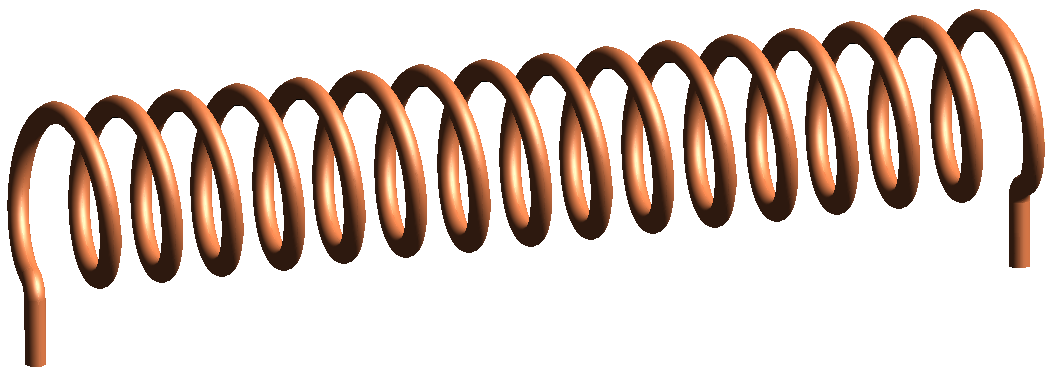
\includegraphics[width=\columnwidth]{Elektro/Elekfig/Solenoid-1.png}
        \caption{Illustration af en solenoide. Kilde: \cite{SolenoidWikipedia2019}}
        \label{fig:solenoide}
    \end{subfigure}
    %
    \hfill
    %
    \begin{subfigure}[t]{.47\textwidth}
        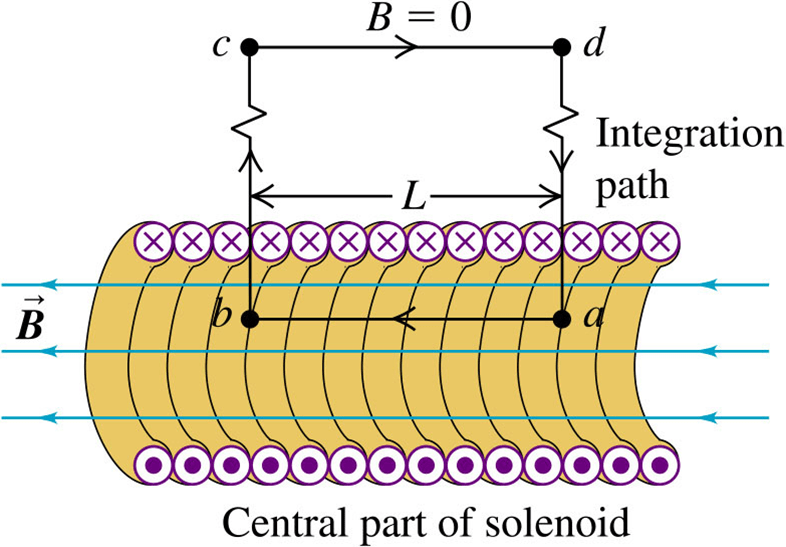
\includegraphics[width=\columnwidth]{Elektro/Elekfig/solenoid.png}
        \caption{Tegning af en solenoide med $n$ vindinger pr. længde, hvori der løber en strøm med strømstyrke $I$. Kilde: \cite{UY1ApplicationsAmpere2015}}
        \label{fig:solenoide_ampere}
    \end{subfigure}
    \caption{ }
\end{figure}
\end{opgave}
\begin{opgave}[3]{Lang lige leder med udstrækning}
    I Magnetostatikafsnittet blev det magnetiske felt fra en uendelig tynd lang lige leder med strømstyrke $I$ bestemt. Situationen ændrer sig en smule, hvis lederen har en endelig tykkelse $R$, og strømstyrken uniformt fordelt over tværsnittet.
    \opg Argumenter for at udregningerne ikke ændrer sig i en afstand $r>R$, hvorfor magnetfeltet er det samme.
    \opg Argumenter for at integralet i Amperes lov er det samme indenfor og udenfor lederen:
    %
    \begin{align}
        \oint \va B \cdot \dd \va l = 2\pi B r,
    \end{align}
    %
    hvor $r$ er afstanden lederens centrum.
    \opg Vis at den indesluttede strøm i tilfældet $r<R$ er
    %
    \begin{align}
        I_\textup{inde} = I \frac{r^2}{R^2}.
    \end{align}
    %
    \opg Brug dette til at vise at
    %
    \begin{align}
        B = \begin{cases}
            \mu_0I/2\pi r, \quad &r>R \\
            \mu_0Ir/2\pi R^2, \quad &r<R
        \end{cases}
        .
    \end{align}
    %
    \opg Skitser funktionen $B(r)$.
    \opg Argumenter kvalitativt for hvordan funktionen $B(r)$ ville se ud hvis lederen var hul med en indre radius $R_0$ og skitser funktionen.
\end{opgave}

\end{document}